\section{Modules, homomorphisms and exact sequences}
\begin{ex}
    If $A$ is an abelian group and $n>0$ an integer such that $na=0$ for all $a\in A$, then $A$ is a unitary $Z_{n}$-module, with the action of $Z_{n}$ on $A$ given by $\bar{k}a=ka$, where $k\in \mathbf{Z}$ and $k\mapsto \bar{k}\in Z_{n}$ under the canonical projection $\mathbf{Z}\to Z_{n}$.
\end{ex}

\begin{answer}
    $\bar{k}, \bar{l}\in Z_{n}$, $k, l\in \mathbf{Z}$ and $a,b\in A$, $(\bar{k}+\bar{l})a=(k+l)a=ka+la=\bar{k}a+\bar{l}a$, $\bar{k}(a+B)=k(a+b)=ka+kb=\bar{k}a+\bar{k}b$. Assume $\bar{kl}=kl\mod n =t$, $\bar{kl}=ta=k(la)=\bar{k}(\bar{l}a)$ since $kl=t+sn, s\in \mathbf{N}$. So $A$ is a $Z_{n}$-module.
\end{answer}

$$ $$

\begin{ex}
    Let $f:A\to B$ be an $R$-module homomorphism.
    \begin{enumerate}[(a)]
        \item $f$ is a monomorphism if and only if for every pair of $R$-module homomorphisms $g,h:D\to A$ such that $fg=fh$, we have $g=h$.
        \item $f$ is an epimorphism if and only if for every pair of $R$-module homomorphisms $k,t:B\to A$ such that $kf=tf$, we have $k=t$.
    \end{enumerate}
\end{ex}

\begin{answer}
    \begin{enumerate}[(a)]
        \item If $f$ is a monomorphism, $f(a)=f(b)$ if and only if $a=b$, so $fg(a)=fh(a)\, \forall a\in D\Rightarrow g(a)=h(a)\, \forall a\in D$, whence $g=h$.
        
        Conversely. Take $D=\mathrm{Ker}f$ and $g:a\mapsto a\in A$, $h:a\mapsto 0\in A$. Then $\forall a\in D$, $fg(a)=fh(a)=0\in B$. This means $D=\{0\}$, so $f$ is a monomorphism.
        \item If $f$ is an epimorphism. $\forall b\in B$, there is $a\in A$ such that $f(a)=b$. So $gf(a)=hf(a)\Rightarrow g(b)=f(b)\, \forall b\in B$, $g=h$.
        
        Conversely. Take $k:b\mapsto b+\mathrm{Im}f$ and $t:b\mapsto -\in B /\mathrm{Im}f$. $\forall a\in A$, $f(a)\in \mathrm{Im}f$ so $kf(a)=\mathrm{Im}f=tf(a)\Rightarrow k=t$. So $\mathrm{Im}f=B$, $f$ is an epimorphism.
    \end{enumerate}
\end{answer}

$$ $$

\begin{ex}
    Let $I$ be a left ideal of a ring $R$ and $A$ an $R$-module.
    \begin{enumerate}[(a)]
        \item If $S$ is a nonempty subset of $A$, then $IS=\{\sum\limits_{i=1}^{n}r_{i}a_{i}|n\in \mathbf{N}^{*}; r_{i}\in I;a_{i}\in S\}$ is a submodule of $A$. Note that if $S=\{a\}$, then $IS=Ia=\{ra|r\in I\}$.
        \item If $I$ is a two-sided ideal, then $A /IA$ is an $R /I$-module with the action of $R /I$ given by $(r+I)(a+IA)=ra+IA$.
    \end{enumerate}
\end{ex}

\begin{answer}
    \begin{enumerate}[(a)]
        \item For any $x\in IS$, $x=\sum\limits_{i=1}^{n}r_{i}a_{i}$ so $rx=r\sum\limits_{i=1}^{n}r_{i}a_{i}=\sum\limits_{i=1}^{n}(rr_{i})a_{i}\in IS$. For any $x,y\in IS$, $x=\sum\limits_{i=1}^{n}r_{i}a_{i}$, $y=\sum\limits_{i=1}^{n'}r_{i}'a_{i}'$. Then $x+y=x=\sum\limits_{i=1}^{n}r_{i}a_{i}+\sum\limits_{i=1}^{n'}r_{i}'a_{i}'\in IS$. $IS$ is a submodule of $A$.
        \item For any $r+I\in R /I$, and $a+IA=A /IA$. $(r+I)(a++IA)=ra+IA\in A /IA$ since $ra\in A$. $\forall r_{1},r_{2}\in R$, $a_{1},a_{2}\in A$. \[\begin{aligned}
            ((r_{1}+I)+(r_{2}+I))(a+IA)&=(r_{1}+r_{2}+I)(a+IA)\\&=(r_{1}a+r_{2}a+IA)\\&=(r_{1}a+IA)+(r_{2}a+IA)
        \end{aligned}\]
        \[\begin{aligned}
            (r+I)((a_{1}+IA)+(a_{2}+IA))&=(r+I)(a_{1}+a_{2}+IA)\\&=ra_{1}+ra_{2}+IA\\&=(ra_{1}+IA)+(ra_{2}+IA)
        \end{aligned}\]
        \[\begin{aligned}
            (r_{1}+I)(r_{2}+I)(a+IA)&=r_{1}r_{2}a+IA\\&=r_{1}(r_{2}a)+IA\\&=(r_{1}+I)(r_{2}a+I)
        \end{aligned}\]
        so $A /IA$ is a submodule of $R /I$.
    \end{enumerate}
\end{answer}

$$ $$

\begin{ex}
    If $R$ has identity, then every unitary cyclic $R$-module is isomorphic to an $R$-module of the form $R /J$, where $J$ is a left ideal of $R$.
\end{ex}

\begin{answer}
    The cyclic unitary module generated by $a$ is $Ra$. We only need to prove $J=\{r|ra=0\in Ra\}$ is an left ideal of $R$. $\forall r'\in R$ and $r\in J$, $r'ra=r'(ra)=r'0=0\in Ra$ so $r'r\in J$. $J$ is a left ideal of $R$. Thus $Ra\cong R /J$.
\end{answer}

$$ $$

\begin{ex}
    If $R$ has identity, then a nonzero unitary $R$-module $A$ is \textbf{simple} if its only submodules are 0 and $A$.
    \begin{enumerate}[(a)]
        \item Every simple $R$-module is cyclic.
        \item If $A$ is simple every $R$-module endomorphism is either the zero map of and isomorphism.
    \end{enumerate}
\end{ex}

\begin{answer}
    \begin{enumerate}[(a)]
        \item Trivial.
        \item For and endomorphism $f$, $\mathrm{Im}f$ is a submodule of $A$, so $f$ is a zero map or an isomorphism.
    \end{enumerate}
\end{answer}

$$ $$

\begin{ex}
    A finitely generated $R$-module need not to be finitely generated as an an abelian group.
\end{ex}

\begin{answer}
    For the polynomial ring with degree less than 3. $\mathrm{Q}_{2}[x]$ is finitely generated  $\mathrm{Q}$-module. But $\mathrm{Q}\subset \mathrm{Q}_{2}[x]$, $\mathrm{Q}_{2}[x]$ is not finitely generated abelian group since $\mathrm{Q}$ is not finitely generated.
\end{answer}

$$ $$

\begin{ex}
    \begin{enumerate}[(a)]
        \item If $A$ and $B$ are $R$-modules, then the set $\mathrm{Hom}_{R}(A,B)$ of all $R$-module homomorphisms $A\to B$ is an abelian group with $f+g$ given on $a\in A$ by $(f+g)(a)=f(a)+g(a)\in B$. The identity element is the zero map.
        \item $\mathrm{Hom}_{R}(A,B)$ is a ring with identity, where multiplication is composition of functions. $\mathrm{Hom}_{R}(A,B)$ is called the \textbf{endomorphism ring} of $A$.
        \item $A$ is a left $\mathrm{Hom}_{R}(A,A)$-module with $fa$ defined to be \[f(a)(a\in A), f\in \mathrm{Hom}_{R}(A,A)\]
    \end{enumerate}
\end{ex}

\begin{answer}
    \begin{enumerate}[(a)]
        \item For any $f,g\in \mathrm{Hom}_{R}(A,B)$, $f+g:=(f+g)(a)=f(a)+g(a)\in B$ and $f+g=g+f$. Take the 0 element as the zero map and the inverse element of $f$ as $-f:a\mapsto -f(a)$. We have $\mathrm{Hom}_{R}(A,B)$ an abelian group.
        \item $\mathrm{Hom}_{R}(A,A)$ is an abelian group. $\forall f,g,h\in \mathrm{Hom}_{R}(A,A)$, \[(fg)h=(f\circ h)\circ h=f\circ g\circ h=f\circ(g\circ h)=f(gh)\]
        \[f\circ(g+h)(a)=f(g(a)+h(a))=f(g(a))+f(h(a))\]
        so $f(g+h)=fg+fh$.
        \[(f+g)\circ h(a)=(f+g)(h(a))=f(h(a))+g(h(a))\]
        so $(f+g)h=fh+gh$. $\mathrm{Hom}_{R}(A,A)$ is a ring and the identity is $1_{A}$ map.
        \item $\forall a\in A$ and $f\mathrm{Hom}_{R}(A,A)$, $fa=f(a)\in A$. For all $a,b\in A$, $f,g\in\mathrm{Hom}_{R}(A,A)$,\[(f+g)a=f(a)+g(a)=fa+ga\]\[f(a+b)=f(a)+f(b)=fa+fb\]\[(fg)a=f(g(a))=f(ga)\]so $A$ is a $\mathrm{Hom}_{R}(A,A)$-module. 
    \end{enumerate}
\end{answer}

$$ $$

\begin{ex}
    Prove that the obvious analogues of Theorem I.8.10 and Corollary I.8.11 are valid for $R$-modules.
\end{ex}

\begin{answer}
    Let $\{f_{i}:G_{i}\to H_{i}|i\in I\}$ be a family of homomorphisms of $R$-module. Let $f:\bigoplus\limits_{i\in I}$ be the map $\bigoplus\limits_{i\in I}G_{i}\to \bigoplus\limits_{i\in I}H_{i}$ given by $\{a_{i}\}\mapsto \{f_{i}(a_{i})\}$. Then $f$ is a homomorphism of $R$-modules such that $f(\bigoplus\limits_{i\in I})\subset \bigoplus\limits_{i\in I}H_{i}$, $\mathrm{Ker}f=\bigoplus\limits_{i\in I}\mathrm{Ker}f_{i}$ and $\mathrm{Im}f=\bigoplus\limits_{i\in I}f_{i}$.

    For any $a_{i},b_{i}\in H_{i}$ with $i\in I$, $f(\{a_{i}\})=\{f_{i}(a_{i})\}$, $f(\{b_{i}\})=\{f_{i}(b_{i})\}$ and $f(\{a_{i}b_{i}\})=\{f_{i}(a_{i}b_{i})\}=\{f_{i}(a_{i})f_{i}(b_{i})\}=\{f(a_{i})\}\{f(b_{i})\}=f(\{a_{i}\})f(\{b_{i}\})$. For any $r\in R$, $f(\{ra_{i}\})=\{f_{i}(ra_{i})\}=\{rf_{i}(a_{i})\}=r\{f_{i}(a_{i})\}=rf(\{a_{i}\})$. Hence $f$ is a well defined homomorphism of $R$-modules. $\{0\}\in \bigoplus\limits_{i\in I}H_{i}$ is the zero element
     of $\bigoplus\limits_{i\in I}H_{i}$, so $\forall \{a_{i}\}\in \mathrm{Ker}f$, $f_{i}(a_{i})=0$. Thus $\mathrm{Ker}f=\bigoplus\limits_{i\in I}\mathrm{Ker}f_{i}$.

     The analogue of Corollary I.8.11 is the obvious corollary of the theorem above.
\end{answer}

$$ $$

\begin{ex}
    If $f:A\to A$ is an $R$-module homomorphism such that $ff=f$, then \[A=\mathrm{Ker}f\oplus\mathrm{Im}f\]
\end{ex}

\begin{answer}
    For the theorem of homomorphisms, $\mathrm{Im}f\cong A /\mathrm{Ker}f$. Suppose $\mathrm{Ker}f\cap \mathrm{Im}f\neq \{0\}$, $a\in \mathrm{Ker}f\cap \mathrm{Im}f$. $a=f(b)$, $f(a)=f(f(b))=f(b)=a=0$, that's contradictory! So $\mathrm{Ker}f\cap \mathrm{Im}f=\{0\}$. $A=\mathrm{Ker}f\oplus\mathrm{Im}f$.
\end{answer}

$$ $$

\begin{ex}
    Let $A,A_{1},\dots, A_{n}$ be $R$-modules. Then $A\cong A_{1}\oplus\cdots\oplus A_{n}$ if and only if for each $i=1,2,\dots,n$ there is an $R$-module homomorphism $\varphi_{i}:A\to A$ such that $\mathrm{Im}\varphi_{i}\cong A_{i}$; $\varphi_{i}\varphi_{j}$ for $i\neq j$; and $\varphi_{1}+\varphi_{2}+\cdots+\varphi_{n}=1_{A}$.
\end{ex}

\begin{answer}
    If $A\cong A_{1}\oplus \cdots\oplus A_{n}$. Let $\pi_{i},\tau_{i}$ be as in Theorem 1.14. Define $\varphi_{i}=\tau_{i}\pi_{i}$. Then $\varphi_{i}\varphi_{j}=0$ for $i\neq j$ and $\sum\limits_{i=1}^{n}=1_{A}$. $\mathrm{Im}\varphi_{i}\cong \pi_{i}(\tau_{i}(A_{i}))=1_{A_{i}}(A_{i})=A_{i}$.

    Conversely. If exist $\varphi_{i}$, $i\in I$ satisfies those conditions. $\varphi_{i}(\varphi_{1}+\cdots+\varphi_{n})=\varphi_{i}$, $\varphi_{i}\varphi_{j}=0$ for $i\neq j$, so $\varphi_{i}\varphi_{i}=\varphi_{i}$. Let $\psi_{i}=\varphi_{i}|\mathrm{Im}\varphi_{i}:\mathrm{Im}\varphi_{i}\to A$. Then $\varphi_{i}\psi_{i}=1_{\mathrm{Im}\varphi_{i}}$ since $\forall \varphi_{i}(a)\in \mathrm{Im}\varphi_{i}$, $\varphi_{i}\psi_{i}(\varphi_{i}(a))=\varphi_{i}(a)$. $\varphi_{i}\psi_{j}=0$ if $i\neq j$. $\sum\limits_{i=1}^{n}\psi_{i}\varphi_{i}=1_{A}$ since $\sum\limits_{i=1}^{n}\varphi_{i}=\sum\limits_{i=1}^{n}\varphi_{i}\varphi_{i}=1_{A}$. From Theorem 1.14, $A\cong \bigoplus\limits_{i=1}^{n}\mathrm{Im}\varphi_{i}$.
\end{answer}

$$ $$

\begin{ex}
    \begin{enumerate}[(a)]
        \item If $A$ is a module over a commutative ring $R$ and $a\in A$, then $\mathcal{O}_{a}=\{r\in R|ra=0\}$ is an ideal of $R$. If $\mathcal{O}_{a}\neq 0$, $a$ is said to be a \textbf{torsion element} of $A$.
        \item if $R$ is an integral domain, then the set $T(A)$ of all torsion elements of $A$.($T(A)$ is called the \textbf{torsion submodule}.)
        \item Show that (b) may be false for a commutative ring $R$, which is not an integral domain.
        
        In (d) - (f) $R$ is an integral domain.
        \item If $f:A\to B$ is an $R$-module homomorphism, then $f(T(A))\subset T(B)$; hence the restriction $f_{T}$ of $f$ to $T(A)$ is an $R$-module homomorphism $T(A)\to T(B)$.
        \item If $0\to A\xrightarrow{f} B\xrightarrow{g} C$ is an exact sequence of $R$-module, then so is $0\to T(A)\xrightarrow{f_T} T(B)\xrightarrow{g_T}T(C)$.
        \item If $g:B\to C$ is an $R$-module epimorphism, then $g_{T}:T(B)\to T(C)$ need not be an epimorphism.
    \end{enumerate}
\end{ex}

\begin{answer}
    \begin{enumerate}[(a)]
        \item Trivial.
        \item For any $a,b\in T(A)$ and $r_{1},r_{2}\in R$ such that $r_{1}a=r_{2}b=0$, $r_{1}r_{2}(a+b)=r_{2}(r_{1}a)+r_{1}(r_{2}b)=0\Rightarrow a+b\in T(A)$. $\forall r\in R$, $r_{1}ra=r(r_{1}a)=0\Rightarrow ra\in T(A)$. $T(A)$ is a submodule of $A$.
        \item Take $R=Z_{6}=\{0,1,2,3,4,5\}$. $R$ itself is an $R$-module and $2,3\in T(R)$, but $2+3=5\notin T(R)$ since $5x=0$ if and only if $x=0$.
        \item We only need to check $\forall a\in T(A)$, $f(a)\in T(B)$. There exist $r\in R$ s.t. $ra=0$, so $f(ra)=rf(a)=f(0)=0$ so $f(a)\in T(B)$, $f(T(A))\subset T(B)$.
        \item If $0\to A\xrightarrow{f} B\xrightarrow{g}C\to 0$ is an exact sequence. $f(A)=\mathrm{Ker}g$, $fg_{T}(a)=0\Rightarrow g_{T}f_{T}(a)=0$. Hence $0\to T(A)\xrightarrow{f_{T}}T(B)\xrightarrow{g_{T}}T(C)\to 0$ is an exact sequence.
        \item $\mathbf{Z}$ itself is a $\mathbf{Z}$-module. $Z_{6}$ is a $\mathbf{Z}$-module as the multiplication given by $a\cdot \bar{b}=\bar{ab}$, $\mathbf{Z}$ has the torsion submodule. $\{0\}$ and $Z_{6}$ has the torsion submodule $\{\bar{0},\bar{2},\bar{3},\bar{4}\}$ which means $f:\mathbf{Z}\to Z_{6}$ cannot form an epimorphism $f_{T}:T(\mathbf{Z})\to T(Z_{6})$.
    \end{enumerate}
\end{answer}

$$ $$

\begin{ex}
    (The Five Lemma). Let
    \begin{figure}[H]\centering
        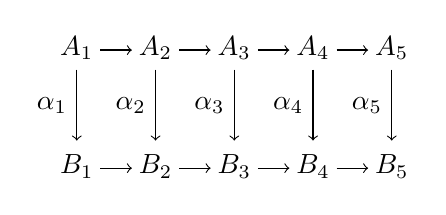
\begin{tikzpicture}
            \node [above] at (0,0) {$B_{1}$};
            \node [above] at (1,0) {$B_{2}$};
            \node [above] at (2,0) {$B_{3}$};
            \node [above] at (3,0) {$B_{4}$};
            \node [above] at (4,0) {$B_{5}$};
            \node [above] at (0,1.5) {$A_{1}$};
            \node [above] at (1,1.5) {$A_{2}$};
            \node [above] at (2,1.5) {$A_{3}$};
            \node [above] at (3,1.5) {$A_{4}$};
            \node [above] at (4,1.5) {$A_{5}$};
            \draw [->] (0.3,0.25) to (0.7,0.25);
            \draw [->] (1.3,0.25) to (1.7,0.25);
            \draw [->] (2.3,0.25) to (2.7,0.25);
            \draw [->] (3.3,0.25) to (3.7,0.25);
            \draw [->] (0.3,1.75) to (0.7,1.75);
            \draw [->] (1.3,1.75) to (1.7,1.75);
            \draw [->] (2.3,1.75) to (2.7,1.75);
            \draw [->] (3.3,1.75) to (3.7,1.75);
            \draw [->] (0,1.5)-- node [left, pos=0.5]{$\alpha_{1}$} (0,0.6);
            \draw [->] (1,1.5)-- node [left, pos=0.5]{$\alpha_{2}$} (1,0.6);
            \draw [->] (2,1.5)-- node [left, pos=0.5]{$\alpha_{3}$} (2,0.6);
            \draw [->] (3,1.5)-- node [left, pos=0.5]{$\alpha_{4}$} (3,0.6);
            \draw [->] (4,1.5)-- node [left, pos=0.5]{$\alpha_{5}$} (4,0.6);
        \end{tikzpicture}
    \end{figure}
    be a commutative diagram of $R$-module homomorphisms, with exact rows. Prove that:
    \begin{enumerate}[(a)]
        \item $\alpha_{1}$ an epimorphism and $\alpha_{2},\alpha_{4}$ monomorphisms $\Rightarrow$ $\alpha_{3}$ is a monomorphism;
        \item $\alpha_{5}$ a monomorphism and $\alpha_{2},\alpha_{4}$ epimorphisms $\Rightarrow$ $\alpha_{3}$ is an epimorphism.
    \end{enumerate}
\end{ex}

\begin{answer}
    Denote all the homomorphisms as following.
    \begin{figure}[H]\centering
        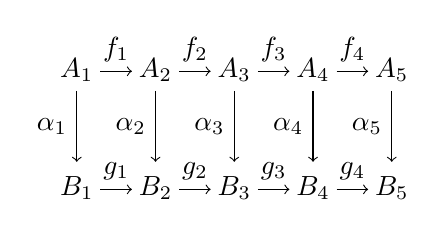
\begin{tikzpicture}
            \node [above] at (0,0) {$B_{1}$};
            \node [above] at (1,0) {$B_{2}$};
            \node [above] at (2,0) {$B_{3}$};
            \node [above] at (3,0) {$B_{4}$};
            \node [above] at (4,0) {$B_{5}$};
            \node [above] at (0,1.5) {$A_{1}$};
            \node [above] at (1,1.5) {$A_{2}$};
            \node [above] at (2,1.5) {$A_{3}$};
            \node [above] at (3,1.5) {$A_{4}$};
            \node [above] at (4,1.5) {$A_{5}$};
            \draw [->] (0.3,0.25)-- node [above, pos=0.5]{$g_{1}$} (0.7,0.25);
            \draw [->] (1.3,0.25)-- node [above, pos=0.5]{$g_{2}$} (1.7,0.25);
            \draw [->] (2.3,0.25)-- node [above, pos=0.5]{$g_{3}$} (2.7,0.25);
            \draw [->] (3.3,0.25)-- node [above, pos=0.5]{$g_{4}$} (3.7,0.25);
            \draw [->] (0.3,1.75)-- node [above, pos=0.5]{$f_{1}$} (0.7,1.75);
            \draw [->] (1.3,1.75)-- node [above, pos=0.5]{$f_{2}$} (1.7,1.75);
            \draw [->] (2.3,1.75)-- node [above, pos=0.5]{$f_{3}$} (2.7,1.75);
            \draw [->] (3.3,1.75)-- node [above, pos=0.5]{$f_{4}$} (3.7,1.75);
            \draw [->] (0,1.5)-- node [left, pos=0.5]{$\alpha_{1}$} (0,0.6);
            \draw [->] (1,1.5)-- node [left, pos=0.5]{$\alpha_{2}$} (1,0.6);
            \draw [->] (2,1.5)-- node [left, pos=0.5]{$\alpha_{3}$} (2,0.6);
            \draw [->] (3,1.5)-- node [left, pos=0.5]{$\alpha_{4}$} (3,0.6);
            \draw [->] (4,1.5)-- node [left, pos=0.5]{$\alpha_{5}$} (4,0.6);
        \end{tikzpicture}
    \end{figure}
    \begin{enumerate}[(a)]
        \item For any $a\in A_{3}$, $\alpha_{3}(a)=0$, we need to show that $a=0$. $g_{3}\alpha_{3}(a)=\alpha_{4}f_{3}(a)=0$, since $\alpha_{4}$ is monomorphism, $f_{3}(a)=0$. So $a\in \mathrm{Ker}f_{3}\Rightarrow a\in \mathrm{Im}f_{2}$. There's $a'\in A_{2}$, $f_{2}(a')=a$, $\alpha_{3}f_{2}(a')=0=g_{2}\alpha_{2}(a')$. So $\alpha_{2}(a')\in \mathrm{Ker}g_{2}=\mathrm{Im}g_{1}$. There is $b''\in B_{1}$, $g_{1}(b'')=\alpha_{2}(a')$. $\alpha_{1}$ is epimorphism so $\exists a''\in A_{1}$, $b''=\alpha_{1}(a'')$, so $g_{1}\alpha_{1}(a'')=\alpha_{2}f_{1}(a'')=\alpha_{2}(a')$. $\alpha_{2}$ is monomorphism so $f_{1}(a'')=a'\in \mathrm{Ker}f_{2}\Rightarrow a=f_{2}(a')=0$.
        \item For any $b\in B_{3}$, we need to show that $b\in \mathrm{Im}\alpha_{3}$. $g_{3}(b)\in B_{4}$, $g_{3}(b)=\alpha_{4}(a')$ for $a'\in A_{4}$ since $\alpha_{4}$ is epimorphism. $g_{4}\alpha_{4}(a')=g_{4}g_{3}(b)=0=\alpha_{5}f_{4}(a')$. $f_{4}a'=0$ cince $\alpha_{5}$ is monomorphism. So there is $a\in A_{3}$, $f_{3}(a)=a'$, $\alpha_{4}f_{3}(a)=g_{3}\alpha_{3}(a)=\alpha_{4}(a')=g_{3}(b)$. $g_{3}(b-\alpha_{3}(a))=0\Rightarrow b-\alpha_{3}(a)\in\mathrm{Ker}g_{3}=\mathrm{Im}g_{2}$. There's $b'\in B_{2}$, $g_{2}(b')=-b+\alpha_{3}(a)$. $\alpha_{2}$ is epimorphism so $\exists a''\in A_{2}$, $\alpha_{2}(a'')=b'$. Consider $\alpha_{3}(a-f_{2}(a''))=\alpha_{3}(a)-\alpha_{3}f_{2}(a'')=-g_{2}\alpha_{2}(a'')+\alpha_{3}(a'')=b$. Thus $b\in \mathrm{Im}\alpha_{3}$, whence $\alpha_{3}$ is epimorphism.
    \end{enumerate}
\end{answer}

$$ $$

\begin{ex}
    \begin{enumerate}[(a)]
        \item If $0\to A\to B\xrightarrow{f} C\to 0$ and $0\to C\xrightarrow{g} D\to D\to E\to 0$ are short exact sequences of modules, then the sequence $0\to A\to B\xrightarrow{gf}D \to E\to 0$ is exact.
        \item Show that every exact sequence may be obtained by splicing together suitable short exact sequences as in (a).
    \end{enumerate}
\end{ex}

\begin{answer}
    \begin{enumerate}[(a)]
        \item The commutative diagram
        \begin{figure}[H]\centering
            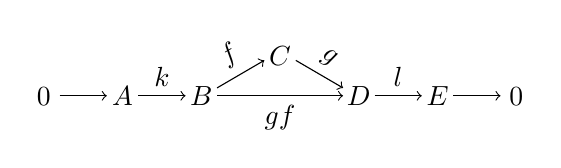
\begin{tikzpicture}
                \node [above] at (0,0) {$0$};
                \node [above] at (1,0) {$A$};
                \node [above] at (2,0) {$B$};
                \node [above] at (4,0) {$D$};
                \node [above] at (5,0) {$E$};
                \node [above] at (6,0) {$0$};
                \node [below] at (3,1) {$C$};
                \draw [->] (0.2,0.25) to (0.8,0.25);
                \draw [->] (1.2,0.25)-- node [above, pos=0.5] {$k$} (1.8,0.25);
                \draw [->] (4.2,0.25)-- node [above, pos=0.5] {$l$} (4.8,0.25);
                \draw [->] (5.2,0.25) to (5.8,0.25);
                \draw [->] (2.2,0.25)-- node [below, pos=0.5] {$gf$} (3.8,0.25);
                \draw [->] (2.2,0.35)-- node [above, pos=0.5, sloped] {$f$} (2.8,0.7);
                \draw [->] (3.2,0.7)-- node [above, pos=0.5, sloped] {$g$} (3.8,0.35);
            \end{tikzpicture}
        \end{figure}
        For any $a\in A$, $k(a)\in \mathrm{Ker}f\Rightarrow fk(a)=0$. $g$ is monomorphism so $\mathrm{Ker}g=0$. Since $gfk(a)=0$, $\mathrm{Im}k\subset \mathrm{Ker}gf$. $\mathrm{Ker}g=0\Rightarrow gf(a)=0$ if and only if $f(a)=0$. $\mathrm{Ker}gf\subset \mathrm{Im}k$. $\mathrm{Im}gf=\mathrm{Im}g$ since $f$ is epimorphism. So $\mathrm{Im}gf=\mathrm{Ker}l$. $0\to A\to B\xrightarrow{gf}D\to E\to 0$ is an exact sequence.
        \item For any finite exact sequence $A_{1}\xrightarrow{f_{1}}A_{2}\xrightarrow{f_{2}}\cdots \xrightarrow{f_{n-1}}A_{n}$. We can add head and tail into it and form
        \[0\to \mathrm{Coker}f_{1}\to A_{1}\xrightarrow{f_{1}}\to A_{2}\xrightarrow{f_{2}}\cdots\xrightarrow{f_{n-1}}A_{n}\to \mathrm{Coim}f_{n-1}\to 0\]
        For any exact sequence which has fragment
        \[A\xrightarrow{f}B\xrightarrow{g}C\xrightarrow{h}D\]
        Consider
        \begin{figure}[H]\centering
            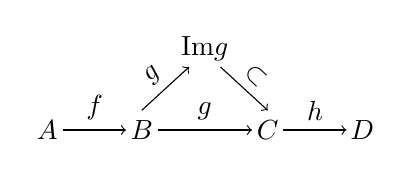
\begin{tikzpicture}
                \node [above] at (0,0) {$A$};
                \node [above] at (1.2,0) {$B$};
                \node [above] at (2.8,0) {$C$};
                \node [above] at (4,0) {$D$};
                \node [above] at (2,1) {$\mathrm{Im}g$};
                \draw [->] (0.2,0.25)-- node [above, pos=0.5] {$f$} (1,0.25);
                \draw [->] (1.4,0.25)-- node [above, pos=0.5] {$g$} (2.6,0.25);
                \draw [->] (3,0.25)-- node [above, pos=0.5] {$h$} (3.8,0.25);
                \draw [->] (1.2,0.5)-- node [above, pos=0.5, sloped] {$g$} (1.8,1.05);
                \draw [->] (2.2,1.05)-- node [above, pos=0.5, sloped] {$\subset$} (2.8,0.5);
            \end{tikzpicture}
        \end{figure}
        $\subset$ is the inclusion map. We can split into $A\xrightarrow{f}B\xrightarrow{g}\mathrm{Im}g\to 0$ and $0\to \mathrm{Im}g\xrightarrow{\subset}C\xrightarrow{h}D$. This provides us a way to split an exact sequence into short exact sequences.
    \end{enumerate}
\end{answer}

$$ $$

\begin{ex}
    Show that isomorphism of short exact sequences is an equivalence relation.
\end{ex}

\begin{answer}
    We check isomorphism of short exact sequence is equivalence relation. $a=0\to A_{1}\to B_{1}\to C_{1}\to 0$, $b=0\to A_{2}\to B_{2}\to C_{2}\to 0$ and $c=0\to A_{3}\to B_{3}\to C_{3}\to 0$.
    \begin{enumerate}
        \item The commutative diagram
        \begin{figure}[H]\centering
            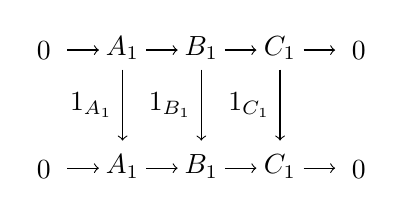
\begin{tikzpicture}
                \node [above] at (0,0) {$0$};
                \node [above] at (1,0) {$A_{1}$};
                \node [above] at (2,0) {$B_{1}$};
                \node [above] at (3,0) {$C_{1}$};
                \node [above] at (4,0) {$0$};
                \node [above] at (0,1.5) {$0$};
                \node [above] at (1,1.5) {$A_{1}$};
                \node [above] at (2,1.5) {$B_{1}$};
                \node [above] at (3,1.5) {$C_{1}$};
                \node [above] at (4,1.5) {$0$};
                \draw [->] (0.3,0.25) to (0.7,0.25);
                \draw [->] (1.3,0.25) to (1.7,0.25);
                \draw [->] (2.3,0.25) to (2.7,0.25);
                \draw [->] (3.3,0.25) to (3.7,0.25);
                \draw [->] (0.3,1.75) to (0.7,1.75);
                \draw [->] (1.3,1.75) to (1.7,1.75);
                \draw [->] (2.3,1.75) to (2.7,1.75);
                \draw [->] (3.3,1.75) to (3.7,1.75);
                \draw [->] (1,1.5)-- node [left, pos=0.5]{$1_{A_{1}}$} (1,0.6);
                \draw [->] (2,1.5)-- node [left, pos=0.5]{$1_{B_{1}}$} (2,0.6);
                \draw [->] (3,1.5)-- node [left, pos=0.5]{$1_{C_{1}}$} (3,0.6);
            \end{tikzpicture}
        \end{figure}
        shows that $a\sim a$ since $1_{A_{1}}$, $1_{B_{1}}$ and $1_{C_{1}}$ are isomorphisms.
        \item If
        \begin{figure}[H]\centering
            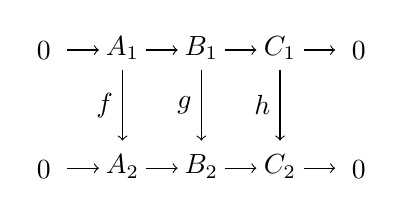
\begin{tikzpicture}
                \node [above] at (0,0) {$0$};
                \node [above] at (1,0) {$A_{2}$};
                \node [above] at (2,0) {$B_{2}$};
                \node [above] at (3,0) {$C_{2}$};
                \node [above] at (4,0) {$0$};
                \node [above] at (0,1.5) {$0$};
                \node [above] at (1,1.5) {$A_{1}$};
                \node [above] at (2,1.5) {$B_{1}$};
                \node [above] at (3,1.5) {$C_{1}$};
                \node [above] at (4,1.5) {$0$};
                \draw [->] (0.3,0.25) to (0.7,0.25);
                \draw [->] (1.3,0.25) to (1.7,0.25);
                \draw [->] (2.3,0.25) to (2.7,0.25);
                \draw [->] (3.3,0.25) to (3.7,0.25);
                \draw [->] (0.3,1.75) to (0.7,1.75);
                \draw [->] (1.3,1.75) to (1.7,1.75);
                \draw [->] (2.3,1.75) to (2.7,1.75);
                \draw [->] (3.3,1.75) to (3.7,1.75);
                \draw [->] (1,1.5)-- node [left, pos=0.5]{$f$} (1,0.6);
                \draw [->] (2,1.5)-- node [left, pos=0.5]{$g$} (2,0.6);
                \draw [->] (3,1.5)-- node [left, pos=0.5]{$h$} (3,0.6);
            \end{tikzpicture}
        \end{figure}
        then we have
        \begin{figure}[H]\centering
            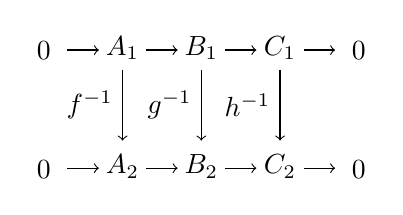
\begin{tikzpicture}
                \node [above] at (0,0) {$0$};
                \node [above] at (1,0) {$A_{2}$};
                \node [above] at (2,0) {$B_{2}$};
                \node [above] at (3,0) {$C_{2}$};
                \node [above] at (4,0) {$0$};
                \node [above] at (0,1.5) {$0$};
                \node [above] at (1,1.5) {$A_{1}$};
                \node [above] at (2,1.5) {$B_{1}$};
                \node [above] at (3,1.5) {$C_{1}$};
                \node [above] at (4,1.5) {$0$};
                \draw [->] (0.3,0.25) to (0.7,0.25);
                \draw [->] (1.3,0.25) to (1.7,0.25);
                \draw [->] (2.3,0.25) to (2.7,0.25);
                \draw [->] (3.3,0.25) to (3.7,0.25);
                \draw [->] (0.3,1.75) to (0.7,1.75);
                \draw [->] (1.3,1.75) to (1.7,1.75);
                \draw [->] (2.3,1.75) to (2.7,1.75);
                \draw [->] (3.3,1.75) to (3.7,1.75);
                \draw [->] (1,1.5)-- node [left, pos=0.5]{$f^{-1}$} (1,0.6);
                \draw [->] (2,1.5)-- node [left, pos=0.5]{$g^{-1}$} (2,0.6);
                \draw [->] (3,1.5)-- node [left, pos=0.5]{$h^{-1}$} (3,0.6);
            \end{tikzpicture}
        \end{figure}
        is also commutative. So $a\sim b\Leftrightarrow b\sim a$.
        \item If
        \begin{figure}[H]\centering
            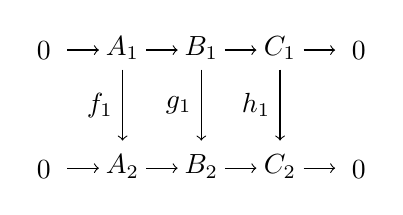
\begin{tikzpicture}
                \node [above] at (0,0) {$0$};
                \node [above] at (1,0) {$A_{2}$};
                \node [above] at (2,0) {$B_{2}$};
                \node [above] at (3,0) {$C_{2}$};
                \node [above] at (4,0) {$0$};
                \node [above] at (0,1.5) {$0$};
                \node [above] at (1,1.5) {$A_{1}$};
                \node [above] at (2,1.5) {$B_{1}$};
                \node [above] at (3,1.5) {$C_{1}$};
                \node [above] at (4,1.5) {$0$};
                \draw [->] (0.3,0.25) to (0.7,0.25);
                \draw [->] (1.3,0.25) to (1.7,0.25);
                \draw [->] (2.3,0.25) to (2.7,0.25);
                \draw [->] (3.3,0.25) to (3.7,0.25);
                \draw [->] (0.3,1.75) to (0.7,1.75);
                \draw [->] (1.3,1.75) to (1.7,1.75);
                \draw [->] (2.3,1.75) to (2.7,1.75);
                \draw [->] (3.3,1.75) to (3.7,1.75);
                \draw [->] (1,1.5)-- node [left, pos=0.5]{$f_{1}$} (1,0.6);
                \draw [->] (2,1.5)-- node [left, pos=0.5]{$g_{1}$} (2,0.6);
                \draw [->] (3,1.5)-- node [left, pos=0.5]{$h_{1}$} (3,0.6);
            \end{tikzpicture}
        \end{figure}
        and
        \begin{figure}[H]\centering
            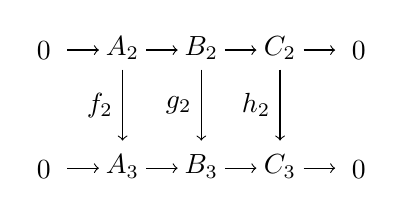
\begin{tikzpicture}
                \node [above] at (0,0) {$0$};
                \node [above] at (1,0) {$A_{3}$};
                \node [above] at (2,0) {$B_{3}$};
                \node [above] at (3,0) {$C_{3}$};
                \node [above] at (4,0) {$0$};
                \node [above] at (0,1.5) {$0$};
                \node [above] at (1,1.5) {$A_{2}$};
                \node [above] at (2,1.5) {$B_{2}$};
                \node [above] at (3,1.5) {$C_{2}$};
                \node [above] at (4,1.5) {$0$};
                \draw [->] (0.3,0.25) to (0.7,0.25);
                \draw [->] (1.3,0.25) to (1.7,0.25);
                \draw [->] (2.3,0.25) to (2.7,0.25);
                \draw [->] (3.3,0.25) to (3.7,0.25);
                \draw [->] (0.3,1.75) to (0.7,1.75);
                \draw [->] (1.3,1.75) to (1.7,1.75);
                \draw [->] (2.3,1.75) to (2.7,1.75);
                \draw [->] (3.3,1.75) to (3.7,1.75);
                \draw [->] (1,1.5)-- node [left, pos=0.5]{$f_{2}$} (1,0.6);
                \draw [->] (2,1.5)-- node [left, pos=0.5]{$g_{2}$} (2,0.6);
                \draw [->] (3,1.5)-- node [left, pos=0.5]{$h_{2}$} (3,0.6);
            \end{tikzpicture}
        \end{figure}
        are commutative. Then
        \begin{figure}[H]\centering
            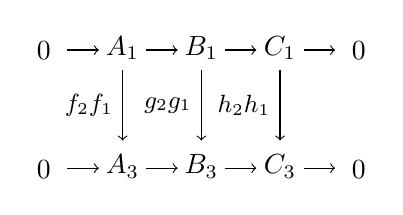
\begin{tikzpicture}
                \node [above] at (0,0) {$0$};
                \node [above] at (1,0) {$A_{3}$};
                \node [above] at (2,0) {$B_{3}$};
                \node [above] at (3,0) {$C_{3}$};
                \node [above] at (4,0) {$0$};
                \node [above] at (0,1.5) {$0$};
                \node [above] at (1,1.5) {$A_{1}$};
                \node [above] at (2,1.5) {$B_{1}$};
                \node [above] at (3,1.5) {$C_{1}$};
                \node [above] at (4,1.5) {$0$};
                \draw [->] (0.3,0.25) to (0.7,0.25);
                \draw [->] (1.3,0.25) to (1.7,0.25);
                \draw [->] (2.3,0.25) to (2.7,0.25);
                \draw [->] (3.3,0.25) to (3.7,0.25);
                \draw [->] (0.3,1.75) to (0.7,1.75);
                \draw [->] (1.3,1.75) to (1.7,1.75);
                \draw [->] (2.3,1.75) to (2.7,1.75);
                \draw [->] (3.3,1.75) to (3.7,1.75);
                \draw [->] (1,1.5)-- node [left, pos=0.5]{\small{$f_{2}f_{1}$}} (1,0.6);
                \draw [->] (2,1.5)-- node [left, pos=0.5]{\small{$g_{2}g_{1}$}} (2,0.6);
                \draw [->] (3,1.5)-- node [left, pos=0.5]{\small{$h_{2}h_{1}$}} (3,0.6);
            \end{tikzpicture}
        \end{figure}
        is also commutative. So $a\sim b, b\sim c\Rightarrow a\sim c$.
    \end{enumerate}
\end{answer}

$$ $$

\begin{ex}
    If $f:A\to B$ and $g:B\to A$ are $R$-module homomorphisms such that $gf=1_{A}$, then $B=\mathrm{Im}f\oplus \mathrm{Ker}g$.
\end{ex}

\begin{answer}
    $gf=1_{A}$ so $f$ is monomorphism and $g$ is epimorphism. So $B /\mathrm{Ker}g\cong \mathrm{Im}g=A\cong A /{0}\cong \mathrm{Im}f$. $\mathrm{Ker}g\cap \mathrm{Im}0=\{0\}$ since $g(\mathrm{Im}f)=A$. Thus $B=\mathrm{Ker}g\oplus\mathrm{Im}f$.
\end{answer}

$$ $$

\begin{ex}
    Let $R$ be a ring and $R^{op}$ its opposite ring. If $A$ is a left $R$-module, then $A$ is a right $R^{op}$-module such that $ra=ar$ for all $a\in A, 4\in R, r\in R^{op}$.
\end{ex}

\begin{answer}
    Trivial.
\end{answer}

$$ $$

\begin{ex}
    \begin{enumerate}[(a)]
        \item If $R$ has an identity and $A$ is an $R$-module, then there are submodules $B$ and $C$ of $A$ such that $B$ is unitary, $RC=0$ and $A=B\oplus C$.
        \item Let $A_{1}$ be another $R$-module, with $A_{1}=B_{1}\oplus C_{1}$ ($B_{1}$ unitary, $RC=0$), If $f:A\to A_{1}$ is an $R$-module homomorphism then $f(B)\subset B_{1}$ and $f(C)\subset C_{1}$.
        \item If the map $f$ of part (b) is an epimorphism, then so are $f|B:B\to B_{1}$ and $f|C:C\to C_{1}$.
    \end{enumerate}
\end{ex}

\begin{answer}
    \begin{enumerate}[(a)]
        \item Let $B=\{1_{R}a|a\in A\}$, $C=\{a\in A|1_{R}a=0\}$. Then $B$ is unitary since $1_{R}(1_{R}a)=1_{R}a$. $RC=0$ since $ra=(r1_{R})a=r(1_{R}a)=0 \forall a\in C$. And $\forall a\in A$, $1_{R}(a-1_{R}a)=0\Rightarrow a-1_{R}a\in C$. So $A=\subset B\oplus C$. Obviously $B\oplus C\subset A$, $A=B\oplus C$.
        \item For any $x=b_{1}+c_{1}\in A_{1}$, $1_{R}x=1_{R}(b_{1}+c_{1})=1_{R}b_{1}$, $B_{1}$ is the maximal unitary submodule and $B_{1}$ contains all unitary elements. $f(B)$ is also unitary since $f(b)=f(1_{R}b)=1_{R}f(b)$ for any $b\in B$. $f(B)\subset B_{1}$.
        
        $C_{1}$ contains all elements $x\in A_{1}$ s.t. $Rx=0$. Since $Rf(c)=f(Rc)=0$ for all $c\in C$, we have $f(C)\subset C_{1}$.
        \item For any $b'\in B'$, we have $f(x)=b'$ since $f$ is epimorphism. Assume $x=b+c$ with $b\in B$ and $c\in C$. $f(x)=f(1_{R}(b+c))=f(1_{R}b)=1_{R}f(b)=f(b)$. So $\exists b\in B$, $f(b)=b'$. $f|B$ is epimorphism. For any $c'\in C$, we have $f(y)=c$. Assume $y=a+d$ with $a\in B$ and $d\in C$. $f(y)=f(1_{R}(a+d))=f(1_{R}a)=0$, so $1_{R}f(a)=0\Rightarrow a=0$. Thus $\exists y=d\in C$, $f(d)=c'$. $f|C$ is epimorphism.
    \end{enumerate}
\end{answer}

$$ $$

\begin{ex}
    Let $R$ be a ring without identity. Embed $R$ in a ring $S$ with identity and charateristic zero as in the proof of Theorem III.1.10. Identify $R$ with its image in $S$.
    \begin{enumerate}[(a)]
        \item Show that every element of $S$ may be uniquely expressed in the form $r1_{S}+n1_{S}(r\in R, n\in \mathbf{Z})$.
        \item If $A$ is an $R$-module and $a\in A$, show that there is a unique $R$-module homomorphism $f:S\to A$ such that $f(1_{S})=a$.
    \end{enumerate}
\end{ex}

\begin{answer}
    \begin{enumerate}[(a)]
        \item Trivial since $S=R\times \mathbf{Z}$.
        \item $S=R1_{S}\oplus\mathbf{Z}1_{S}$. Let $f(r1_{S}+n1_{S})=ra+na$, then $f(1_{S})=a$ and $f$ is a well defined homomorphism of modules. If there exists another $g$ s.t. $g(1_{S})=a$, $\forall r1_{S}+n1_{S}\in S$, $g(r1_{S}+n1_{S})=rg(1_{S})+ng(1_{S})=ra+na=f(r1_{S}+n1_{S})$. So $g=f$.
    \end{enumerate}
\end{answer}